\documentclass[
	ngerman,
	twoside,
	pdfa=false,
	ruledheaders=section,%Ebene bis zu der die Überschriften mit Linien abgetrennt werden, vgl. DEMO-TUDaPub
	class=report,% Basisdokumentenklasse. Wählt die Korrespondierende KOMA-Script Klasse
	thesis={type=Hausarbeit},%bachelor},% Dokumententyp Thesis, für Dissertationen siehe die Demo-Datei DEMO-TUDaPhd
	accentcolor=2c,%3d,% Auswahl der Akzentfarbe
	custommargins=false,% Ränder werden mithilfe von typearea automatisch berechnet
	marginpar=false,% Kopfzeile und Fußzeile erstrecken sich nicht über die Randnotizspalte
	%BCOR=5mm,%Bindekorrektur, falls notwendig
	parskip=half-,%Absatzkennzeichnung durch Abstand vgl. KOMA-Sript
	fontsize=12pt,%Basisschriftgröße laut Corporate Design ist mit 9pt häufig zu klein
	% logofile=images/tuda_logo.pdf, %Falls die Logo Dateien nicht installiert sind
]{tudapub}

%%%%%%%%%%%%%%%%%%%%%%%%%%%%
% Download des TU-Logos
%%%%%%%%%%%%%%%%%%%%%%%%%%%%
% https://download.hrz.tu-darmstadt.de/protected/CE/TUDa_LaTeX/tuda_logo.pdf
% Der Pfad zum Logo kann als "logofile" angegeben werden.

%%%%%%%%%%%%%%%%%%%
% Sprachanpassung & Verbesserte Trennregeln
%%%%%%%%%%%%%%%%%%%
\usepackage[english, main=ngerman]{babel}
\usepackage[autostyle]{csquotes}% Anführungszeichen vereinfacht
\usepackage{microtype}

%%%%%%%%%%%%%%%%%%%
% Literaturverzeichnis
%%%%%%%%%%%%%%%%%%%
\usepackage[backend=biber,style=numeric]{biblatex}   % Literaturverzeichnis
\addbibresource{literature.bib}
% WICHTIG!! je nach Version ist es nötig, manuell auf Biber zum Erzeugen des Literaturverzeichnisses umzustellen: Optionen --> TexStudio konfigurieren... --> Erzeugen --> StandardBibliograhieprogramm --> Biber

%%%%%%%%%%%%%%%%%%%
% Paketvorschläge Tabellen
%%%%%%%%%%%%%%%%%%%
%\usepackage{array}     % Basispaket für Tabellenkonfiguration, wird von den folgenden automatisch geladen
\usepackage{tabularx}   % Tabellen, die sich automatisch der Breite anpassen
%\usepackage{longtable} % Mehrseitige Tabellen
%\usepackage{xltabular} % Mehrseitige Tabellen mit anpassarer Breite
\usepackage{booktabs}   % Verbesserte Möglichkeiten für Tabellenlayout über horizontale Linien

%%%%%%%%%%%%%%%%%%%
% Paketvorschläge Mathematik
%%%%%%%%%%%%%%%%%%%
\usepackage{mathtools} % erweiterte Fassung von amsmath
\usepackage{amssymb}   % erweiterter Zeichensatz
\usepackage{siunitx}   % Einheiten

%%%%%%%%%%%%%%%%%%%%%%
% Pseudocode
%%%%%%%%%%%%%%%%%%%
\usepackage[linesnumbered,lined,boxruled]{algorithm2e} % Package für Pseudocode
\usepackage{listings}

%%%%%%%%%%%%%%%%%%%
% Plotting und Grafik
%%%%%%%%%%%%%%%%%%%
\usepackage{tuda-pgfplots} % Package für Plotting with TUDa mods
\usepackage{graphicx}

%%%%%%%%%%%%%%%%%%%
% Sonstiges
%%%%%%%%%%%%%%%%%%%
\usepackage{blindtext} % Package für Blindtext
\usepackage{caption}
\usepackage{hyperref}

\begin{document}
	\title{WACE SoSe24 Hausarbeit Team03}
	\subtitle{Kurs: Wissenschaftliches Arbeiten im CE}
	%\author[V. Name]{Vorname Name} %optionales Argument ist die Signatur,
	\author[Karakoc, Rosenhagen, Tanase]{Aykut Karakoc, Christian Rosenhagen und Bogdan Tanase} %optionales Argument ist die Signatur,
	%\reviewer{Gutachter 1 \and Gutachterin 2} %Gutachten

	%Diese Felder erden untereinander auf der Titelseite platziert.
	%\department{ce} % Das Kürzel wird automatisch ersetzt und als Studienfach gewählt, siehe Liste der Kürzel im Dokument.
	\institution{
		% Fügt das CE-Logo über dem Schriftzug ein
		{\color{accentcolor}
\includegraphics[width=0.9\linewidth]{images/ce_logo_black.pdf}}
		% oder etit-Logo: 
		%\includegraphics[width=0.9\linewidth]{images/etit_logo}
	}
	
	%\submissiondate{\today}
	%\examdate{\today}

	%	\tuprints{urn=1234,printid=12345}
	%	\dedication{Für alle, die \TeX{} nutzen.}

	\maketitle
	\pagenumbering{gobble} % Seitenzahlen angezeigt, startet ab dem Inhaltsverzeichnis

	%%%%%%%%%%%%%%%%%%%
	%Eigenständigkeitserklärung (bei Abschlussarbeiten BSc/MSc erforderlich, nicht hier bei dieser WACE-Hausarbeit!)
	%%%%%%%%%%%%%%%%%%%
	%\affidavit

	%%%%%%%%%%%%%%%%%%%
	%Abstract / Kurzzusammenfassung
	%%%%%%%%%%%%%%%%%%%
    \section*{Abstract}

Diese Hausarbeit beschäftigt sich mit der Approximation der Differentiation und Integration, um die Anwendung dieser in der Praxis zu untersuchen. Zuerst werden Praxisbeispiele der Integral- und Differentialrechnung erläutert sowie die spezifischen Probleme, die bei diesen Verfahren auftreten können. Im zweiten Teil wird die Differentiation untersucht beginnend mit der Erklärung der finiten Differenzenmethoden und deren Genauigkeit. In diesem Abschnitt wird über die Finite-Differenzen-Methode(FDM) und deren Umsetzung in Python eingegangen anhand einer Simulation der Blechverformung. Der letzte Teil fokussiert sich auf die Newton-Cotes-Formeln(NCF) sowie die verschiedenen Varianten, wie beispielsweise die Trapez-, Simpson-, $\frac{3}{8}$- und Milne-Regel. Diese wird auch als Code in Python implementiert und präsentiert, wie die Schnittkräfte eines Tragwerks berechnet und geplottet werden.

	%%%%%%%%%%%%%%%%%%%
	%Inhaltsverzeichnis 
	%%%%%%%%%%%%%%%%%%%
	\tableofcontents % Erstellte ein Inhaltsverzeichnis
	
	\cleardoublepage
	\pagenumbering{arabic} % Seitenzahlen angezeigt, startet ab dem Inhaltsverzeichnis
	\setcounter{page}{1} % Setzt den Seitenzahlenzähler auf 1

%%%%%%%%%%%%%%%%%%%%%%%%%%%%%%%%%%%%%%%%%%%%%%%%%%%%%%%%%%%%%%%%%%%%%%%%%%%%%%%%%%%%%%%%%%%%%%%%%%

	% INHALT, am Besten ausgelagert in eigene Files/Kapitel und dann mit \include{Unterordner/Filename} eingefügt, sorgt für bessere Übersichtlichkeit und Fehlersuche. Einzelne Dateien sind aktuell im Ordner Sections abgelegt. 

    \chapter{Wo spielen Differentiation und Integration in der Praxis eine Rolle und was sind die Schwierigkeiten dabei?}

\section{Praxisanwendungen Integralrechnung}

In vielen Bereichen spielt die praktischen Anwendung der Integralrechnung oft eine wichtige Rolle. In den Ingenieurswissenschaften oder in der Physik wird die Integralrechnung unter anderem zum Berechnen verschiedenster Flächen unter willkürlichen Kurven und zum Berechnen von Volumina genutzt \textsc{\cite{ARD-Alpha-Integral}} \textsc{\cite{Anwendung-Integrale}}. Des Weiteren kann man mit der Integralrechnung in der Mechanik verschiedene physikalische Größen, wie zum Beispiel die Schnittgröße berechnen \textsc{\cite{TM-Schnittgroessen}}. Die Integralrechnung spielt nicht nur in der Physik und den Ingenieurswissenschaften eine wichtige Rolle, sondern auch in der Statistik und Wahrscheinlichkeitsrechnung. Hierbei werden Integrale genutzt um den Erwartungswert einer Zufallszahl zu berechnen \textsc{\cite{MatheIngVertiefung_S.520f}}. Allerdings spielt nicht nur in den sehr mathematischen Bereichen, sondern auch beispielsweise in Umweltwissenschaften und in der Geographie. In diesen Bereichen wird die Integralrechnung dafür genutzt, um zum Beispiel die Durchflussmenge anhand der Geschwindigkeit über einen gewissen Querschnitt zu berechnen. \textsc{\cite[S. 22]{Hydrologie_S.22}}

\section{Praxisanwendung Differentialrechnung}

Die Differentialrechnung wird ebenfalls, wie die Integralrechnung, in vielen Bereichen von Ingeneieurswissenschaften genutzt um beispielsweise die Änderungsrate an einem exakten Punkt einer Kurve festzustellen, dies kann somit unter anderem die Geschwindigkeit oder das Wachstum zu einer bestimmten Zeit sein. \textsc{\cite{ElektroAbleitung}}

\section{Schwierigkeiten bei der Integral- und Differentialrechnung}

Die Schwierigkeiten oder Problematik bei der Integralrechnung liegt darin, dass bei numerischen Integrationsmethoden, wie der Sehnen-Trapez oder bei der Simpson-Methode, eine niedrige Genauigkeit herrscht \textsc{\cite[S. 205]{WingMatheProblem_S218}}. Des Weiteren haben viele Funktionen in der Praxis keine einfachen, beziehungsweise keine bekannten Stammfunktionen. Dies erschwert die Integration dieser Funktion erheblich.
Die Schwierigkeiten bei der Differentialrechnung bestehen darin, dass zum einen, wie bei der Integralrechnung auch, die Funktionen nicht immer einfach sind und zum Anderen, dass Studenten oder Schüler oft die Steigung nicht direkt mit der Ändereungsrate in Verbindung setzen \textsc{\cite[S. 78]{AbleitungMatheWingWis_S78}}. 

	
	\chapter{Differentiation}


\section{Wann und wozu verwendet man die finite Differenz?}

Die finite Differenz wird auf numerische Funktionen angewandt, die als Folge dargestellt werden und sich nur schwer analytisch differenzieren lassen. Sie wird verwendet, um die Ableitung von abgetasteten Daten zu finden, für die die erzeugende Funktion nicht bekannt ist.

\subsection{Vorwärtsdifferenz}

Die Vorwärtsdifferenz verwendet die Stichproben an einem Netzpunkt und den nächsten (vorwärts) gleichabständigen Analysepunkten, um die Ableitung am Netzpunkt zu berechnen. Die Fehlerschranke $O(h^2)$ beschreibt, dass der Fehler bzw. die Abweichung linear mit der Schrittweite anwächst. Das bedeutet: je kleiner $O(h^2)$, umso genauer ist 
\[ \frac{y_{k+1} - y_k}{h}\]
was die Annäherung der Ableitung beschreibt\textsc{\cite[S. 273]{Differentiationsformen}}.


\subsection{Rückwärtsdifferenz}

Die Rückwärtsdifferenz verwendet die Stichproben an einem Netzpunkt und den vorherigen (rückwärtigen) gleichmäßig beabstandeten Punkten, wie im Folgenden 

\[\frac{y_k - y_{k-1}}{h} \text{,}\]um die Ableitung zu berechnen\textsc{\cite[S. 273]{Differentiationsformen}}.

\subsection{Zentraldifferenz}
\label{sec:Zentraldifferenz}

Die Zentraldifferenz verwendet sowohl Vorwärts- als auch Rückwärts-Stichproben zur Berechnung der Ableitung am angegebenen Netzpunkt. Hier werden Taylorreihen höherer Ordnung genutzt, um mit $h < 1$ und 
\[
\frac{y_{k+1} - y_{k-1}}{2h}
\]
die Abweichung gering zu halten\textsc{\cite[S. 273]{Differentiationsformen}}.

Durch diese verschiedenen Annäherungen können Funktionen, die schwer analytisch abzuleiten sind, besser und genauer differenziert werden.

\section{Detaillierte Beschreibung und Genauigkeit}


\subsection{Erster Schritt zur numerischen Lösung}

Der erste Schritt zur numerischen Lösung erfordert die Diskretisierung des Lösungsgebiets. Dazu ist die Definition eines numerischen Gitters notwendig.


\subsection{Gitterstruktur bei Finite-Differenzen (FD) Diskretisierungsverfahren}

Das Gitter ist lokal strukturiert. Jeder Gitterknoten dient als Ursprung eines lokalen Koordinatensystems, wobei die Achsen des lokalen Koordinatensystems mit den Gitterlinien übereinstimmen.


\subsection{Eigenschaften und Anordnung der Gitterlinien}

Die Gitterlinien der gleichen Familie (z.B. $x = \text{const.}$ und $y = \text{const.}$) schneiden sich nicht. Gitterlinien unterschiedlicher Familien schneiden sich nur einmal. In drei Dimensionen schneiden sich drei Gitterlinien in jedem Knoten und bilden dort einen eindeutigen Schnittpunkt; diese Linien schneiden sich an keinem anderen Punkt.

\subsection{Genauigkeit}

Je geringer die Abstände der Gitterknoten sind, desto kleiner ist die entsprechende Abweichung der Annäherung der numerischen Lösung. Siehe in \ref{fig:Gitterknoten-Abstände}.

\begin{figure}[h]
    \centering
    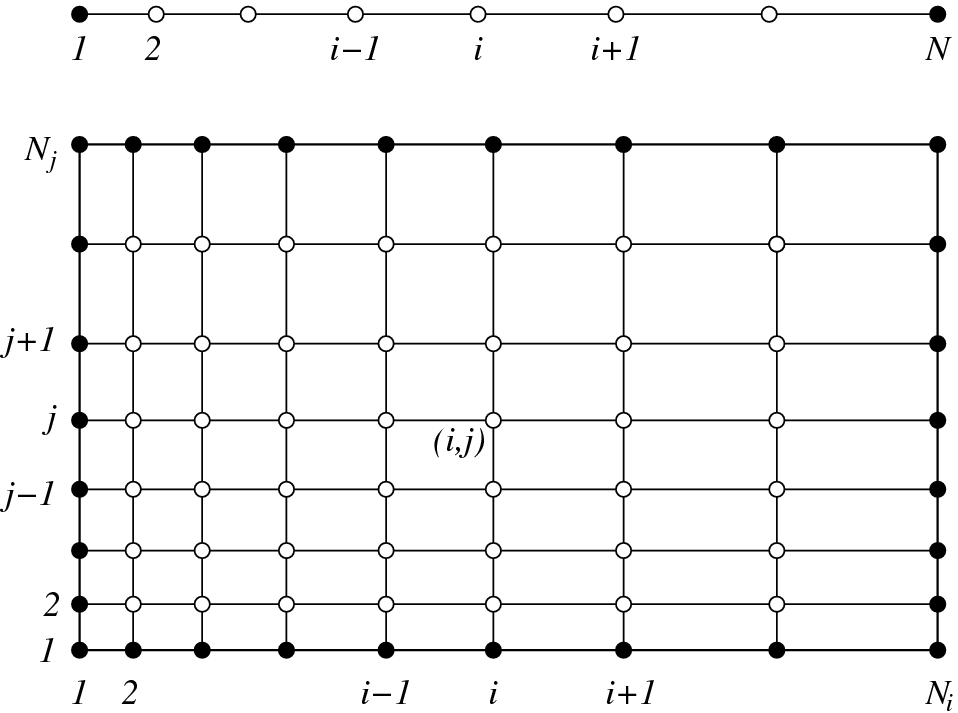
\includegraphics[scale=0.35]{images/Gitterknoten.png}
    \caption{Abstände der Gitterknoten}
    \label{fig:Gitterknoten-Abstände}
\end{figure}

\section{Praxisbeispiel FDM: Bezug zu Computer Engineering (CE)}

Dieses Praxisbeispiel zeigt die Anwendung der Finite-Differenzen-Methode (FDM) zur Berechnung der Wärmeleitung in dreidimensional geformten Blechkörpern\textsc{\cite{Praxisbeispiel_1}}.

\subsection{Herausforderungen bei der Simulation von Blechumformvorgängen}

Die Simulation von Blechumformvorgängen wird häufig mithilfe der Finite-Elemente-Methode (FEM) durchgeführt, wobei diese Simulationen meist isotherm erfolgen. Das bedeutet, dass dabei konstante Temperaturbedingungen angenommen werden. In der Praxis treten jedoch häufig gekoppelte thermisch-mechanische Effekte auf, die bei solchen isothermen Annahmen nicht berücksichtigt werden können. Dies führt zu numerischen Schwierigkeiten und ungenauen Ergebnissen.

\subsection{Vorteile der Finite-Differenzen-Methode (FDM)}

Im Gegensatz zur Finite-Elemente-Methode (FEM) wird die Finite-Differenzen-Methode (FDM) häufig zur Lösung von Wärmeleitungsproblemen eingesetzt. Dabei bietet die FDM mehrere Vorteile gegenüber der FEM:

Eine der Hauptstärken der FDM liegt in ihrer einfacheren Implementierung. Die Methode ist oft weniger komplex zu programmieren als die FEM, was sie besonders für Anwendungsbereiche attraktiv macht, in denen schnelle und unkomplizierte Lösungen gefragt sind.

Ein weiterer Vorteil der FDM ist ihre höhere Effektivität bei der Lösung von Wärmeleitungsproblemen. Die Methode kann in vielen Fällen effizienter und schneller zu Ergebnissen führen, was sie für bestimmte technische und physikalische Anwendungen besonders geeignet macht.


\subsection{Beschränkungen und Weiterentwicklungen der FDM}

Ein wesentlicher Nachteil der herkömmlichen FDM ist ihre Beschränkung auf einfache Geometrien, was ihre Anwendung auf komplexe Strukturen einschränkt. Um dieses Problem zu überwinden, wurde eine neue Variante der FDM entwickelt, die es ermöglicht, die Wärmeleitung in komplex geformten dreidimensionalen Blechen zu berechnen.

\subsection{Parametrisierung und Modellannahmen}

Die neue FDM nutzt eine geeignete Parametrisierung der Mittelfläche des Bleches, was eine effektive Lösung des Wärmeleitungsproblems erlaubt. Dabei wird die Annahme getroffen, dass die Bleche eine sehr geringe Dicke im Vergleich zu ihren anderen Abmessungen haben. Dies vereinfacht die mathematische Modellierung und reduziert den Rechenaufwand.

\subsection{Kopplung mit der Finite-Elemente-Methode (FEM)}

Ein bedeutender Vorteil der neuen FDM besteht darin, dass sie einfach mit der FEM gekoppelt werden kann. Diese Kopplung ermöglicht die simultane Simulation des Umformprozesses und der Wärmeleitung, was zu präziseren und realistischeren Ergebnissen führt. Durch die Kombination der Stärken beider Methoden können sowohl die mechanischen als auch die thermischen Effekte während des Umformprozesses berücksichtigt werden.

\subsection{Anwendungsbeispiele}

Diese neue Methode kann in verschiedenen industriellen Anwendungen eingesetzt werden, insbesondere in der Automobil- und Luftfahrtindustrie, wo die genaue Kontrolle der Temperatur während der Blechumformung entscheidend für die Qualität des Endprodukts ist. Die verbesserte Genauigkeit und Effizienz der neuen FDM tragen dazu bei, die Produktionsprozesse zu optimieren und die Materialeigenschaften gezielt zu beeinflussen.

\section{Implementation der FDM in Python}

\subsection{Vorgehen}
\label{sec:ImplFDM}

Zunächst soll das vorhin erwähnte Praxisbeispiel anhand eines Python-Programms mithilfe der \texttt{Numpy}- und \texttt{Matplotlib}-libraries implementiert werden, das die Finite-Differenzen-Methode (FDM) zur Berechnung der Wärmeleitung in einem dreidimensionalen Blechkörper verwendet. Der folgende Code zeigt die Implementierung der Methoden zur Berechnung der Deformation und der Temperaturverteilung, sowie die Visualisierung der Ergebnisse.

\subsection{Deformations- und Temperaturberechnung}

Die Berechnung der Deformation und der Temperaturverteilung erfolgt anhand der vorher beschriebenen Methoden. Dabei wird die Klasse \texttt{Derivative} (siehe \ref{lst:DerivativeClass}) aus dem Code-Abschnitt zur Approximation von Ableitungen verwendet, also die FDM.

\subsection{Python-Code für die \texttt{Derivative}-Klasse}
Nun wird die \texttt{Derivative}-Klasse näher betrachtet.

\subsubsection{Code der \texttt{Derivative}-Klasse}

Die  \texttt{Derivative}-Klasse bietet Methoden zur Berechnung der numerischen Ableitung einer Funktion mittels der Finite-Differenzen-Methode (FDM). Hier ist der vollständige Python-Code:

\begin{lstlisting}[language=Python, caption={Vollständiger Code der Derivative-Klasse}, label={lst:DerivativeClass}]
    import numpy as np
    from typing import Callable
    
    class Derivative:
        @staticmethod
        def of_order_1(
            f: Callable[[np.ndarray], np.ndarray],
            x: np.ndarray,
            h: float
        ) -> np.ndarray:
            assert h != 0
            return (f(x + h) - f(x - h)) / (2 * h)
    
        @staticmethod
        def of_order_2(
            f: Callable[[np.ndarray], np.ndarray],
            x: np.ndarray,
            h: float
        ) -> np.ndarray:
            assert h != 0
            return (f(x + h) - 2 * f(x) + f(x - h)) / (h * h)
\end{lstlisting}

\subsection{Erklärung der \texttt{Derivative}-Klasse und deren Methoden}

\paragraph{Klasse \texttt{Derivative}}

Die \texttt{Derivative}-Klasse bietet eine statische Methode zur numerischen Berechnung der ersten Ableitung einer Funktion. Sie verwendet die zentrale Differenzenmethode um die Ableitung an einer gegebenen Stelle zu approximieren.

\subsubsection{Methode \texttt{of\_order\_1}}

\paragraph{Parameter:}
\begin{itemize}
    \item \texttt{f}: Eine Funktion, von der die numerische Ableitung berechnet werden soll. Die Funktion sollte ein \texttt{np.ndarray} als Eingabe akzeptieren und ein \texttt{np.ndarray} als Ausgabe zurückgeben.
    \item \texttt{x}: Ein \texttt{np.ndarray}, das die Punkte enthält, an denen die Ableitung berechnet werden soll.
    \item \texttt{h}: Ein \texttt{float}, das die Schrittweite für die Finite-Differenzen-Methode angibt.
\end{itemize}

\paragraph{Rückgabewert:}
\begin{itemize}
    \item \texttt{np.ndarray}: Die numerisch berechnete erste Ableitung der Funktion an den angegebenen Punkten.
\end{itemize}

\paragraph{Funktionsweise:}
Die Methode \texttt{of\_order\_1} aus \ref{lst:DerivativeClass} berechnet die erste Ableitung einer Funktion \texttt{f} an den Punkten \texttt{x} mit einer Schrittweite \texttt{h}. Dies erfolgt durch die zentrale Differenzenmethode, welche in \ref{sec:Zentraldifferenz} numerisch dargestellt wird. Außerdem wird vorrausgesetzt, dass \texttt{h} nicht Null sein darf, da dadurch eine Nulldivision verhindert wird. Folglich wird die Formel

\[ f'(x) \approx \frac{f(x + h) - f(x - h)}{2h} \]

in diesem Kontext angewendet, da das $y$ an Index $k$ den Funktionswert an einer Stelle $x$ entspricht. Wird $k$ erhöht, nimmt die Funktion den Wert am nächsten Schritt an, also bei $x + h$. Dies gilt analog, für den Fall, wenn $k$ verkleinert wird.

Zusätzlich gibt es in \ref{lst:DerivativeClass} eine weitere statische Methode zur Berechnung der zweiten Ableitung einer Funktion. Diese Methode wird in der Implementierung des Kontexts nicht verwendet.

\subsubsection{Methode \texttt{of\_order\_2}}

\paragraph{Parameter:}
\begin{itemize}
    \item \texttt{f}: Eine Funktion, von der die numerische Ableitung berechnet werden soll. Die Funktion sollte ein \texttt{np.ndarray} als Eingabe akzeptieren und ein \texttt{np.ndarray} als Ausgabe zurückgeben.
    \item \texttt{x}: Ein \texttt{np.ndarray}, das die Punkte enthält, an denen die Ableitung berechnet werden soll.
    \item \texttt{h}: Ein \texttt{float}, das die Schrittweite für die Finite-Differenzen-Methode angibt.
\end{itemize}

\paragraph{Rückgabewert:}
\begin{itemize}
    \item \texttt{np.ndarray}: Die numerisch berechnete zweite Ableitung der Funktion an den angegebenen Punkten.
\end{itemize}

\paragraph{Funktionsweise:}
Die Methode \texttt{of\_order\_2} aus \ref{lst:DerivativeClass} berechnet die zweite Ableitung einer Funktion \texttt{f} an den Punkten \texttt{x} mit einer Schrittweite \texttt{h}. Dies erfolgt durch die zentrale Differenzenmethode der zweiten Ableitung, welche einen ähnlichen Aufbau wie die erste hat

\[f''(x) \approx \frac{f(x + h) - 2f(x) + f(x - h)}{h^2}\text{.}\]


\subsection{Python-Code für die Berechnung und Visualisierung}

\paragraph{Anwendungsbeispiel: Simulation der Blechverformung:}
Es wird angenommen, dass eine glatte Blechplatte im Zentrum verformt wird und die Temperaturverteilung über die Oberfläche simuliert werden soll. Der folgende Python-Code zeigt die Implementierung der Methoden zur Berechnung der Deformation und der Temperaturverteilung, sowie die Visualisierung der Ergebnisse. Es ist anzumerken, dass das Beispiel nur reale Maßnahmen annähert und nur als Darstellung für eine Mögliche Nutzung der FDM zur Berechnung der Steigung an den gewünschten Punkten.

\begin{lstlisting}[language=Python, caption={l1 und l2}, label={lst:linFunctions}]
    def l1(x: np.ndarray) -> np.ndarray:
        return 2.5 * x + 3.75


    def l2(x: np.ndarray) -> np.ndarray:
        return -2.5 * x + 3.75
\end{lstlisting}

\texttt{l1} und \texttt{l2} sind lineare Funktionen, die als Hilfe zur Modellierung des verformten Blechsstücks dienen. Betrachtet man den Querschnitt von \ref{fig:MetalSheetDeformation} auf der xz-Ebene bilden die Funktionen die zwei nicht parallelen Seiten eines Trapezes. 

\begin{lstlisting}[language=Python, caption={Deformationsfunktion}, label={lst:deformFunction}]
    def deformation_function(x: np.ndarray) -> np.ndarray:
        z = np.zeros_like(x)
        mask1 = (-1.5 < x) & (x < -1.3)
        mask2 = (-1.3 <= x) & (x <= 1.3)
        mask3 = (1.3 < x) & (x < 1.5)
    
        z[mask1] = l1(x[mask1])
        z[mask2] = 0.5
        z[mask3] = l2(x[mask3])
    
        return z
\end{lstlisting}

\texttt{deformation\_function} kombiniert die Funktionen aus \ref{lst:linFunctions} zur Modellierung der gesamten Verformung des Blechs. Es wird die \texttt{z}-Koordinate zurückgegeben.

\begin{lstlisting}[language=Python, caption={Temperaturfunktion}, label={lst:tempFunction}]
    def temperature_function(x: np.ndarray, z: np.ndarray) -> np.ndarray:
        h = 0.01
        gradient = np.abs(Derivative.of_order_1(deformation_function, x, h)) / 2.5
        temperature = gradient - z
        temperature[(-1.3 <= x) & (x <= 1.3)] = 0.4
        temperature = 1000 * temperature + 20
        return temperature
\end{lstlisting}

\texttt{temperature\_function} berechnet die Temperaturverteilung basierend auf der Verformung. Sie verwendet die Methode \texttt{of\_order\_1} der \texttt{Derivative}-Klasse (siehe \ref{lst:DerivativeClass}) zur Approximation der Ableitung. Die obere Fläche des Blechs bleibt konstant bei einer Temperatur, wärend die schiefen Flächen eine konstante Temperaturverteilung, die abhängig von der Höhe \texttt{z} sind, abbilden. Die Temperatur wird auf einen realistischen Bereich normalisiert.

\begin{lstlisting}[language=Python, caption={Plotten des Verformungsverfahren}, label={lst:PlotMetalDeformation}]
    def plot_simulation_metal_deformation():
        x = np.linspace(-5, 5, 500)
        y = np.linspace(-5, 5, 100)
        x, y = np.meshgrid(x, y)
    
        z = deformation_function(x)
    
        temperature = temperature_function(x, z)
    
        ls = LightSource(azdeg=315, altdeg=45)
        rgb = ls.shade(z, cmap=cm.jet, vert_exag=1, blend_mode='overlay')
    
        fig = plt.figure(figsize=(10, 6))
        ax = fig.add_subplot(111, projection='3d')
    
        surf = ax.plot_surface(
            x,
            y,
            z,
            rstride=1,
            cstride=1,
            facecolors=plt.cm.jet(temperature / 1000),
            linewidth=0,
            antialiased=True,
            shade=False
        )
    
        ax.set_xlabel('x')
        ax.set_ylabel('y')
        ax.set_zlabel('z')
    
        ax.set_zlim(0, 2)
    
        ax.set_title(...)
    
        plt.subplots_adjust(right=0.8)
    
        cbar_ax = fig.add_axes([0.85, 0.15, 0.03, 0.7])
        m = plt.cm.ScalarMappable(cmap=plt.cm.jet)
        m.set_array(temperature)
        fig.colorbar(m, cax=cbar_ax)
    
        ax.view_init(elev=30, azim=135)
    
        plt.show()
\end{lstlisting}
Die Funktion \texttt{plot\_simulation\_metal\_deformation} erstellt ein 3D-Oberflächendiagramm der Verformung mit der entsprechenden Temperaturverteilung. Die Abbildung \ref{fig:MetalSheetDeformation} zeigt den Plot dieser Funktion an. Es wird eine Farbskala verwendet, welche die Temperatur an den Stellen anzeigt, die benötigt wurde, um die Verformung durchzuführen. Das Temperaturintervall reicht von 20°C bis circa 900°C. Man erkennt  Beleuchtungseffekte werden verwendet, um die Visualisierung zu verbessern.

Schließlich wird die Methode \texttt{plot\_simulation\_metal\_deformation} aufgerufen:
\begin{lstlisting}
    plot_simulation_metal_deformation()
\end{lstlisting}

\begin{figure}[h]
    \centering
    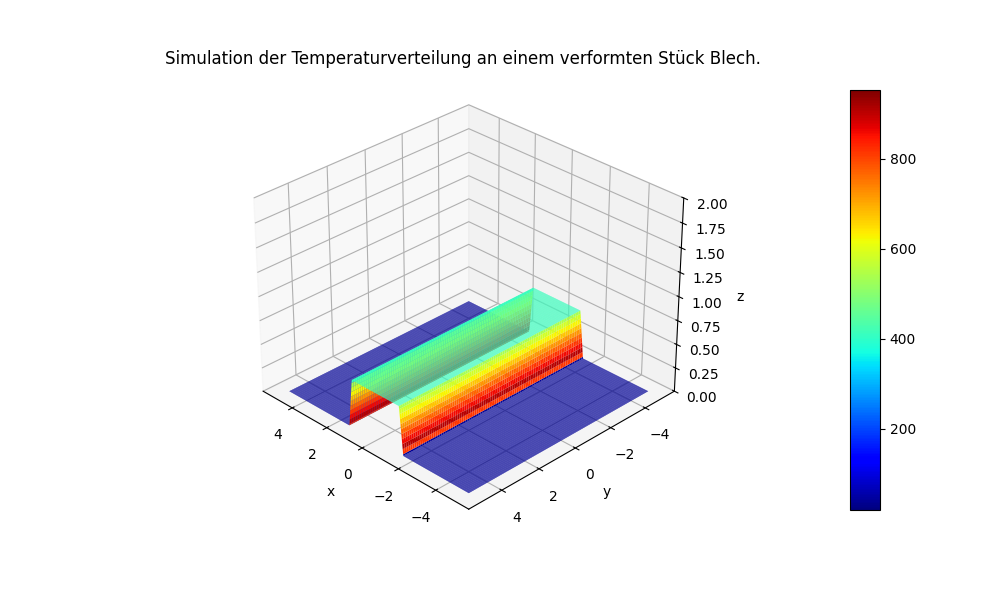
\includegraphics[width=\textwidth]{images/metal_sheet_deformation.png}
    \caption{Verformung und Temperaturverteilung einer Blechplatte}
    \label{fig:MetalSheetDeformation}
\end{figure}

\paragraph{Beobachtung: }
Die nicht verformten Stellen, für \texttt{x<=-1.5} und \texttt{x>=1.5} haben \texttt{z=0}, wurden daher nicht verändert und bleiben bei Raumtemperatur. Zwischen \texttt{-1.5<x<1.5} wird der beschriebene Verlauf deutlich, wie die Temperatur in Abhängigkeit der Steigung und der Höhe sich verändert. 

\subsection{Fazit}
Die Nutzung der FDM bei der Blechverformungen hilft, die Steigung für funktionale Verläufe bei der Verformung auszurechnen, um dafür den Temperaturaufwand zu berechnen. Die Umsetzung der Formel in Code ist simpel und führt zu nahen Approximationen für eine klein gewählte Schrittweite $h$.

Alternativ hätte man auch den plastischen Umformgrad analysieren und plotten können, für den auch die Steigung oder die Krümmung an bestimmten Punkten verwendet wird, wofür der Code aus \ref{lst:DerivativeClass} geeignet ist.
	
	\chapter{Newton-Cotes-Formel}



\section{Einleitung und Zielsetzung}

Das Ziel dieser Arbeit ist die wahrscheinlichkeitstheoretische Herleitung und Begründung der Integrationsformeln von Newton-Cotes. Es wird detailliert untersucht, wie Integrale durch eine lineare Kombination von Funktionswerten an äquidistanten Punkten angenähert werden können. Die Güte dieser Annäherung wird anhand der mittleren quadratischen Abweichung gemessen, die ein Maß für die Genauigkeit der Integration darstellt.

\subsection{Theoretische Grundlagen}

In dieser Arbeit wird ein stationärer stochastischer Prozess $\xi(t)$ verwendet, der durch den Erwartungswert $E[\xi(t)] = 0$ und die Varianz $E[\xi^2(t)] = 1$ charakterisiert ist. Der stochastische Prozess dient der Analyse der Fehlerabschätzung und der Bestimmung optimaler Koeffizienten für die Integrationsformeln\textsc{\cite[S. 190]{Newton-Cotes-Formeln}}.

\subsection{Mathematische Herleitung}

Als Mass für die Güte der Näherung wollen wir den Erwartungswert $E[\eta^2]$
benutzen. Bei vorgegebener Korrelationsfunktion ist $h$ und damit auch $E[\eta^2]$
eine Funktion der Schrittweite $h$ und der Koeffizienten $a_i$ Die Formel zur Berechnung der mittleren quadratischen Abweichung
\[
E[\eta^2] = 2 \int_0^{2nh} S(t) dt - 2 \sum_{i = -n}^{+n} a_i \{ S((n + i)h) + S((n-i)h) \} + \sum_{k,i = -n}^{+n} a_k a_i R((i-k)h)
\]
hat das Ziel die Koeffizienten $a_i$ so zu bestimmen, dass der Fehler $E[\eta^2]$ minimiert wird \textsc{\cite[S. 191] {Newton-Cotes-Formeln}}.

\subsection{Minimierung und Ergebnisse}

Es wird gezeigt, dass die minimalen Lösungen der Koeffizienten $a(i)$ den Koeffizienten der Newton-Cotes-Formeln entsprechen. Die Fehlerabschätzungen für diese optimalen Koeffizienten sind vergleichbar mit den Fehlerabschätzungen der Newton-Cotes-Formeln. Eine Taylor-Entwicklung der Koeffizienten bestätigt zudem die Übereinstimmung mit den Newton-Cotes-Koeffizienten.

\section{Versionen von Newton-Cotes}

\subsection{Trapez-Regel}
\label{sec:Trapez}
Die Trapezregel mit der Gewichtung \( [\frac{1}{2} \text{,} \frac{1}{2}] \) \textsc{\cite[S. 342] {Gewichte}} ist durch ihr Intervall auf alle Natürlichen Zahlen anwendbar \textsc{\cite[S. 6] {Trapezregel}}. Die lineare Interpolation an den Intervallenden kann durch
\[  t_{k-1}\] 
bestimmt werden. 
Für die summierte Treapezregel gilt

\[ T(h)=h\cdot(\frac{1}{2} f(a)+f_{t1}+...+f_{t_{n-1}}+\frac{1}{2} f(b)) \text{.}\]

\subsection{Simpson-Regel}
\label{sec:Simpson}
Durch die Gewichtung
\([ \frac{1}{3} \text{,} \frac{4}{3} \text{,}  \frac{1}{3} ]\) mit dem Wert \(n\) = 2
der Simpsonregel wird die numerische Integration über ein Intervall $[a,b]$ approximiert\textsc{\cite[S. 342] {Gewichte}}. Diese Gewichte stammen aus der Quadraturformel für Parabeln und führen zu einer präziseren Näherung im Vergleich zu einfacheren Methoden wie der Trapezregel. Konkret bedeutet dies, dass die Funktion $f(x)$ an den Endpunkten $a$ und $b$ sowie am Mittelpunkt \[{\frac{a + b}{2}} \] evaluiert wird, wobei die Funktionswerte mit den entsprechenden Gewichten multipliziert werden.

Die Simpson-Regel lautet

\begin{equation}
    \label{eq:SimpsonRegel}
    \int_a^b f(x) dx \approx \frac{b - a}{6} [f(a)+4f(\frac{a + b}{2})+f(b)] \text{,}\tag{Simpson Regel}
\end{equation}

wenn ein einfaches Integral \([a, b]\) vorliegt\textsc{\cite[S. 17] {Simpsonregel/Milneregel}}.

\subsection{\(\frac{3}{8}\)-Regel}
\label{sec:3/8}
Die \(\frac{3}{8}\)-Regel mit der Gewichtung \( [\frac{3}{8} \text{,}\frac{9}{8} \text{,}\frac{9}{8} \text{,}\frac{3}{8}]\), dem gekürzten Wert $n$ = 3 \textsc{\cite[S. 342] {Gewichte}} und der Form

\[ \int_a^b f(x) dx \approx (b-a) [w_0f_0 + w_1f_1 + w_2f_2 + w_3f_3]\]

wird angewendet, indem das Intervall $[a, b]$ in $n$ Teilintervalle geteilt wird, wobei $n$ ein Vielfaches von 3 sein muss.

\subsection{Milne-Regel}
\label{sec:Milne}
Die Milne-Regel mit der Gewichtung \( [\frac{7}{90} \text{,} \frac{32}{90} \text{,} \frac{12}{90} \text{,} \frac{32}{90} \text{,} \frac{7}{90}] \) \textsc{\cite[S. 342] {Gewichte}}
erhält man durch die Formel
\[ \int_a^b f(x) dx \approx \frac{b - a}{90} \cdot (7f(x_0) + 32f(x_1) + 12f(x_2) + 32f(x_3) + 7f(x_4))\]
\textsc{\cite[S. 19] {Simpsonregel/Milneregel}}.

\subsection{Weddle-Regel}
\label{sec:Weddle}
Die Weddle-Regel mit der Gewichtung \( [\frac{41}{840} \text{,} \frac{216}{840} \text{,} \frac{27}{840} \text{,} \frac{272}{840} \text{,} \frac{27}{840} \text{,} \frac{216}{840} \text{,} \frac{41}{840}] \) \textsc{\cite[S. 342] {Gewichte}} mit der Formel
\[ Q_a^b (f) := (b - a) \sum_{i=0}^{n0} \sigma_i f(x_i)\] 

\textsc{\cite[S. 5] {Weddleregel}} erzeugt den Fehler \[ \frac{9}{1400}h^9f^{(9)} (\hat{x}) \text{.} \]


%%%%%%%%%%%%%%%%%%%%%%%%%%%%%%%%%%%%%%%%%%%%%%%%%%%%%%%%%%%%%%%%%%%%%%%%%%%%%%%%%%%%%%%%%%%%%%%%%%%%%%%%%%%%%%%%%%%%%%%%%%%%%%%%%%%%%%%%%%%%%%%%%%%%%%%%%%
%%%%%%%%%%%%%%%%%%%%%%%%%%%%%%%%%%%%%%%%%%%%%%%%%%%%%%%%%%%%%%%%%%%%%%%%%%%%%%%%%%%%%%%%%%%%%%%%%%%%%%%%%%%%%%%%%%%%%%%%%%%%%%%%%%%%%%%%%%%%%%%%%%%%%%%%%%
%%%%%%%%%%%%%%%%%% Simpson-Formel, Varianten sowie Unterschiede und wo welche Simpson Formel sinnvoll ist %%%%%%%%%%%%%%%%%%%%%%%%%%%%%%%%%%%%%%%%%%%%%%%%

\section{Simpson-Formel, Varianten sowie Unterschiede und wo welche Simpson Formel sinnvoll ist}

\subsection{Varianten}

Bei der Simpson Regel gibt es vier verschiedene Varianten, welche nochmal in zwei Kategorien aufgeilt werden können. Man kann es in die \(\frac{1}{3}\)-Formeln und die \(\frac{3}{8}\)-Formeln unterteilen. Diese kann man dann wiederrum in die Einfache Simpson-\(\frac{1}{3}\)-Formel und die Zusammengesetzte Simpson-\(\frac{1}{3}\)-Formel, sowie die Einfache-\(\frac{3}{8}\)-Formel und die Zusammengesetzte Simpson-\(\frac{3}{8}\)-Formel unterteilen \textsc{\cite[S. 342]{SimpsonVarianten}}  \textsc{\cite[S. 327]{BasicNumMath}}.


\subsection{Unterschiede}\label{sec:Unterschiede}

Bei den Unterschieden kann man ebenfalls wieder in die zwei Kategorien \(\frac{1}{3}\)-Formel und \(\frac{3}{8}\)-Formel unterteilen. Die Einfache Simpson-\(\frac{1}{3}\)-Formel kann man für ein einzelnes Intervall benutzen, welches in zwei gleich große Teile geteilt wurde. Die Zusammengesetzte Simpson-\(\frac{1}{3}\)-Formel kann man dahingegen für ein Intervall nutzen, welches in mehrere gleich große Teile geteilt wurde, wobei die Anzahl durch zwei teilbar sein muss. Bei den \(\frac{3}{8}\)-Formeln ist das so ähnlich, bis auf enen kleinen Unterschied. Die Einfache-\(\frac{3}{8}\)-Formel nutzt man für ein einzelnes Intervall, welches in drei gleich große Teile geteilt wurde und die Zusammengesetzte Simpson-\(\frac{3}{8}\)-Formel nutzt man für ein Intervall, das in mehrere gleich große Teile geteilt wurde, allerdings muss die Anzahl der Teile hierbei durch drei teilbar sein \textsc{\cite[S. 310]{NumMathe}} \textsc{\cite[S. 180]{NumMethodsScienceEng}}.


\subsection{Unter welchen Bedingungen bzw. Anforderungen ist welche Simpson Formel sinnvoll}

Im allgemeinen dienen die Simpson-Formeln dazu, eine höhere Genauigkeit zu erreichen als beispielsweise mit der Rechtecks- oder Trapezberechnung. \textsc{\cite[S. 310]{NumMathe}} Sofern die Abstände der Punkte gleichmäßig sind, kann man Formeln, wie die Simpson-Formeln, höherer Ordnung anwenden. Sowohl die \(\frac{1}{3}\)-Formel und die \(\frac{3}{8}\)-Formel haben die gleiche Genauigkeit. Man kann die Simpson-Formeln allerdings nicht nutzen, wenn die Punkte nicht gleichmäßig vertielt sind \textsc{\cite[S. 186]{NumMethodsScienceEng}}. Wie bei den Unterschieden \ref{Unterschiede} erwähnt, kann man die \(\frac{1}{3}\)-Formel dafür benutzen, um eine Fläche in einem Intervall zu berechnen, welche aus einer geraden Anzahl von Teilintervallen besteht. Hierbei muss man allerdings darauf achten, dass die Einfache Simpson-\(\frac{1}{3}\)-Formel nur zwei Teilintervalle haben darf, dafür aber die Zusammengesetzte Simpson-\(\frac{1}{3}\)-Formel aus mehreren Teilintervallen bestehen darf, diese Anzahl aber durch zwei teilbar sein muss. Bei der \(\frac{3}{8}\)-Formel ist das ähnlich, nur das man nicht die Zahl zwei nimmt sondern drei. Die Einfache Simpson-\(\frac{3}{8}\)-Formel muss aus drei Teilintervallen bestehen und die Zusammengesetzte Simpson-\(\frac{3}{8}\)-Formel muss aus einer Anzahl an Teilintervallen bestehen, welche durch drei teilbar ist \textsc{\cite[S. 180]{NumMethodsScienceEng}} \textsc{\cite[S. 186]{NumMethodsScienceEng}}. 

\section{Implementation der Newton-Cotes-Formeln in Python}

\subsection{Vorgehen}
Die Approximation der Integration mit den Newton-Cotes-Formeln soll nun per Code näher betrachtet werden. Hierzu werden, wie in \ref{sec:ImplFDM}, die Python-libraries \texttt{Numpy} und \texttt{Matplotlib} verwendet.

Das Verfahren wird anhand der Schnittgrößen aus der Technischen Mechanik erklärt. Das Beispiel (\ref{fig:ExampleInternalForce})\footnote{Entnommen aus \href{https://pickedshares.com/technische-mechanik-2-uebung-10-traeger-mit-dreieckfoermiger-streckenlast/}{https://pickedshares.com/technische-mechanik-2-uebung-10-traeger-mit-dreieckfoermiger-streckenlast/}} bildet einen, durch eine Linienlast $q_0$ belasteter Träger, welcher an einer Einspannung $A$ gelagert wurde. Der Träger hat die Länge $l$. Es wird ein Koordinatensystem angelegt, mit der horizontalen $x$-Achse, welche nach rechts positiv ist und die vertikale $z$-Achse, welche nach unten positiv ist. Der Ursprung des Koordinatensystems liegt im Lager $A$.

\begin{figure}[h]
    \centering
    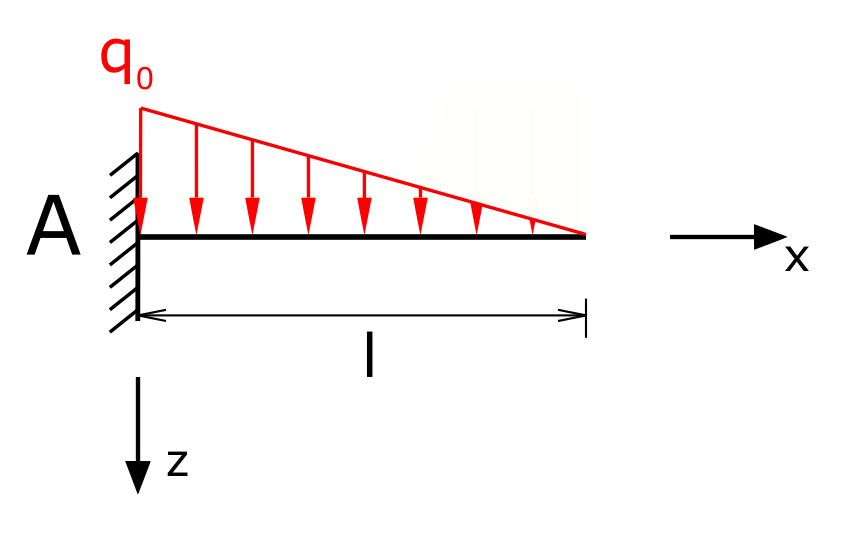
\includegraphics[scale = 0.5]{images/example_internal_force.png}
    \caption{Träger an einem Festlager mit Länge $l$ und Streckenlast $q_0$}
    \label{fig:ExampleInternalForce}
\end{figure}

\subsection{Aus Streckenlast zur Querkraft und Moment}
 Ziel ist es den Querkraft- und Momentenverlauf als Graphen darzustellen. Dazu werden die verschiedenen Varianten der Newton-Cotes-Formeln(NCF), um das Integral zu approximieren, verwendet, welche im Verlauf der Implementierung erläutert werden.

Zur Darstellung der Graphen werden Zahlenbeispiele für die konstanten Größen verwendet. Es wird angemommen, die Länge des Trägers $l$ sei 10 Meter und die Streckenlast $q_0$ entspreche 2 Newton pro Meter.

Der lineare Verlauf lässt sich durch die Gleichung

\begin{equation}
    \label{eq:Streckenlast}
    q(x) = \frac{q_0 (l - x)}{l}\tag{eq1}
\end{equation}

ermitteln. 
Der Querkraft- und Momentverlauf lassen sich dann durch

\begin{equation}
    \label{eq:Querkraft}
    Q(x) = - \int q(x) dx\tag{eq2}
\end{equation}

und

\begin{equation}
    \label{eq:Moment}
    M(x) = \int Q(x) dx\tag{eq3}
\end{equation}

errechnen.

\subsection{Python-Code für die \texttt{NewtonCotes}- und \texttt{SimpsonRule}-Klasse}
Nun werden die \texttt{NewtonCotes}- und \texttt{SimpsonRule}-Klasse näher betrachtet.

\paragraph{Code der \texttt{NewtonCotes}-Klasse}

Die \texttt{NewtonCotes}-Klasse bietet Methoden zur numerischen Berechnung von Integralen mittels der NCF. Es beinhaltet nur die ersten vier Formeln, also von \ref{sec:Trapez} bis \ref{sec:Milne}. Hier ist der vollständige Python-Code:

\begin{lstlisting}[language=Python, caption={Vollständiger Code der NewtonCotes-Klasse}, label={lst:NewtonCotesClass}]
    from typing import Callable
    import numpy as np
    
    class NewtonCotes:
        weightOptions = [
            np.array([1, 1]) * 1 / 2,  #trapezoidal rule
            np.array([1, 4, 1]) * 1 / 3,  #simpson rule
            np.array([1, 3, 3, 1]) * 3 / 8,  #3/8 rule
            np.array([7, 32, 12, 32, 7]) * 2 / 45,  #milne rule
        ]
    
        def __init__(self, n: int):
            assert 0 < n < 5 and isinstance(n, int)
            self.n = n
            self.weight = self.weightOptions[n - 1]
    
        def calculate_integral(
             self,
             f: Callable[[float], float],
             a: float,
             b: float
            ) -> float:
            A = 0
            h = (b - a) / self.n
            for i in range(self.n + 1):
                xi = a + i * h
                A += self.weight[i] * f(xi)
            A *= h
            return A
\end{lstlisting}

\paragraph{Code der \texttt{SimpsonRule}-Klasse}

Die \texttt{SimpsonRule}-Klasse ist eine spezielle Unterklasse der \texttt{NewtonCotes}-Klasse, die die Simpson-Regel zur numerischen Integration verwendet. Hier ist der vollständige Python-Code:

\begin{lstlisting}[language=Python, caption={Vollständiger Code der SimpsonRule-Klasse}, label={lst:SimpsonRuleClass}]
from typing import Callable
import numpy as np
from Code.Approximation_Integral
        .Newton_Cotes.NewtonCotes import NewtonCotes

class SimpsonRule(NewtonCotes):
    def __init__(self, node_count=10):
        super().__init__(2)
        assert node_count > 0
        assert node_count % 2 == 0
        self.node_count = node_count

    def calculate_integral_composite(
         self,
         f: Callable[[float], float],
         a: float,
         b: float
        ) -> float:
        h = (b - a) / self.node_count
        A = f(a) + f(b)
        for i in range(1, self.node_count):
            xi = a + i * h
            if i % 2 == 0:
                A += 2 * f(xi)
            else:
                A += 4 * f(xi)
        return A * h / 3

    def calculate_integral_simple(
         self,
         f: Callable[[float], float],
         a: float,
         b: float
        ) -> float:
        h = (b - a) / 6
        return h * (f(a) + f(b) + 4 * f((a + b)/2))
\end{lstlisting}

\subsection{Erklärung der Klassen und deren Methoden}

\paragraph{\texttt{NewtonCotes}-Klasse}
Das Attribut \texttt{weightOptions} zeigt die verschiedenen Gewichte der NCF. Das Gewicht \texttt{weight}, welches zur Berechnung des Integrals benutzt wird, wird durch die Anzahl an Knoten bestimmt.

Passend dazu ist die Methode \texttt{\_\_init\_\_} der Konstruktor des Objekts, der die Anzahl an Knoten \texttt{n} als Parameter annimmt. Der Code beinhaltet nur die ersten vier Formeln, deshalb kann \texttt{n} maximal 4 sein.

Die Methode \texttt{calculate\_integral} ermittelt die Fläche zwischen einer Funktion \texttt{f} und der $x$-Achse im Intervall \texttt{[a, b]}.

\paragraph{Parameter:}
\begin{itemize}
    \item \texttt{f}: Der Integrant, der eine Funktion ist. Diese sollte einen \texttt{float}-Wert annehmen und sowohl zurückgeben.
    \item \texttt{a}: ein \texttt{float}, der die untere Grenze des Intervalls angibt
    \item \texttt{b}: ein \texttt{float}, der die obere Grenze des Intervalls angibt
\end{itemize}

\paragraph{Rückgabewert:}
\begin{itemize}
    \item \texttt{float}: Die resultierende Fläche
\end{itemize}

\paragraph{Funktionsweise:}
Der Algorithmus bestimmt für jedes iterierte $x_i$, welches die Stellen der einzelnen Knoten sind, den Funktionswert und multipliziert diesen mit dem jeweiligen Gewicht. Alle auf dieser Weise ermittelten Werte werden summiert und mit dem Abstand zwischen den einzelnen Knoten \texttt{h} multipliziert.

\paragraph{\texttt{SimpsonRule}-Klasse}
Die \texttt{SimpsonRule}-Klasse vererbt die \texttt{NewtonCotes}-Klasse. Dadurch wird im Konstruktor der \texttt{SimpsonRule}-Klasse die Superklasse aufgerufen mit dem Parameter \texttt{n=2}, da diese der Simpson-Regel entspricht. Der Konstruktor von dieser Klasse besitzt einen optionalen Parameter \texttt{node\_count}, der standarmäßig auf $10$ gesetzt wird. Dieser beschreibt die Anzahl der Knoten, die benutzt werden, um das Integral zu approximieren. Die Anzahl muss gerade sein, wie in \ref{sec:Unterschiede} schon erwähnt wurde.

Die \texttt{calculate\_integral\_composite}-Methode kann stetig zusammengesetzte Intervalle benutzen, das heißt es ist abhängig vom Attribut \texttt{node\_count}, um das Integral anzunähern.

\paragraph{Parameter und Rückgabewert}
Diese können analog aus der \texttt{calculate\_integral}-Methode der Superklasse\texttt{NewtonCotes} entnommen werden.

\paragraph{Funktionsweise:}
Die Funktionswerte an den Randstellen von $x$ haben keine Gewichtung. Für jedes gerade $x_i$ wird der Funktionswert an dieser Stelle mit der Gewichtung $\frac{2}{3}$ und jedes ungerade mit $\frac{4}{3}$ multipliziert. Diese Werte werden miteinander addiert und mit dem Abstand \texttt{h} multipliziert.

Die \texttt{calculate\_integral\_simple}-Methode approximiert das Integral nur für ein einfaches Intervall \texttt{[a, b]}, das heißt es ist nicht abhängig von \texttt{node\_count}.

\paragraph{Parameter und Rückgabewert}
Diese können analog aus der \texttt{calculate\_integral}-Methode der Superklasse\texttt{NewtonCotes} entnommen werden.

\paragraph{Funktionsweise:}
Die Formel aus \ref{eq:SimpsonRegel} wird übernommen und die Fläche wird zurückgegeben.

\subsection{Anwendung der Newton-Cotes-Formeln zur Bestimmung der Schnittgrößen}

Zunächst wird die \texttt{InternalForces}-Klasse näher betrachtet, die zur Veranschaulichung des Beispiels eines gelagerten Trägers(Abbildung: \ref{fig:ExampleInternalForce}) und die Verwendung der zuvor erwähnten Klassen \texttt{NewtonCotes}(\ref{lst:NewtonCotesClass}) und \texttt{SimpsonRule}(\ref{lst:SimpsonRuleClass}).

Zur Bestimmung der Schnittgrößen (Querkraft $Q(x)$ und Moment $M(x)$) des belasteten Trägers werden die oben implementierten Klassen verwendet und die Konstanten $q_0$ und $l$ eingeführt. Es wird ein Objekt der Klasse \texttt{NewtonCotes} erstellt mit dem Parameter für \texttt{n = 3}. Dies entspricht der $\frac{3}{8}$-Regel. Zusätzlich wird ein Objekt der Klasse \texttt{SimpsonRule} mit dem optionalen Parameter \texttt{node\_count=100}, für eine bessere Approxmierung des Integrals.

\begin{lstlisting}[language=Python]
    import numpy as np
    import matplotlib.pyplot as plt
    from Code.Approximation_Integral
            .Newton_Cotes.SimpsonRule import SimpsonRule
    from Code.Approximation_Integral
            .Newton_Cotes.NewtonCotes import NewtonCotes
    
    l = 10  #Meter
    q_0 = 2  #Newton/Meter
    newtonCotes = NewtonCotes(3)
    simpson = SimpsonRule(node_count=100)
\end{lstlisting}

Es wird die Funktion für die Streckenlast \texttt{q(x)}, welche analog zur Formel für $q(x)$ aus \ref{eq:Streckenlast} implementiert wurde, erstellt.
Für die Querkraft \texttt{Q(x)} wird nach \ref{eq:Querkraft} das negative Integral von \texttt{q(x)} und das Integral davon für das Moment \texttt{M(x)} nach \ref{eq:Moment}.

\begin{lstlisting}[language=Python, label={lst:Func}]
    def q(x: float) -> float:
        return (q_0 * (l - x)) / l
    
    
    def Q(x: float) -> float:
        return -1 * simpson.calculate_integral_composite(q, x, l)
    
    
    def M(x: float) -> float:
        return simpson.calculate_integral_simple(Q, x, l)
\end{lstlisting}

In der Methode \texttt{single\_value\_integral} wird die $\frac{3}{8}$ - Regel aus \ref{lst:NewtonCotesClass} zur Berechnung der Querkraft $Q(x)$ mithilfe des Integrals von der Streckenlast $q(x)$ im Intervall 0 bis 5 benutzt. Diese Methode zeigt, die Annäherung des Integrals und den tatsächlichen, wenn man das zuvor ausgerechnete Integral benutzt.

\begin{lstlisting}[language=Python]
    def single_value_integral():
        integral_with_trapezoidal = newtonCotes.calculate_integral(q, 0, 5)
        approximated_result = (((q_0 * l) / 4) - integral_with_trapezoidal)
        print(f"Approx: {approximated_result}")
        print(f"Tatsaechlich: {Q(5) - Q(0)}")
\end{lstlisting}

Die vollständige Ausgabe, die hier aus Platzgründen(Formaierung) nicht angezeigt wurde, sieht so aus:

\begin{lstlisting}[language=Python]
Console:
    Angenaehertes Integral bei Q(5) - Q(0) mit Trapezregel: 7.5 N
    Tatsaechliches Integral bei Q(5) - Q(0): 7.5 N
\end{lstlisting}

Anschließend wird der ganze Verlauf der Schnittgrößen als drei Graphen mithilfe von \texttt{Matplotlib} in der Methode \texttt{plot\_internal\_forces}. Es wird ein \texttt{Numpy}-Array für \texttt{x} von \texttt{0} bis \texttt{l} erstellt, also den Verlauf von $x$ über das Tragwerk mit der Länge $l$. Die einzelnen Werte der Funktionen werden mit den vorherig erläuterten Methoden (\ref{lst:Func}) berechnet. Die einzelnen Funktionen werden schließlich geplottet.

\begin{lstlisting}
    def plot_internal_forces():
        x = np.linspace(0, l, 100)
    
        q_values = np.array([q(i) for i in x])
        Q_values = np.array([Q(i) for i in x])
        M_values = np.array([M(i) for i in x])
    
        fig, (ax1, ax2, ax3) = plt.subplots(3, 1, figsize=(10, 6))
    
        ax1.plot(x, q_values, label=r'Streckenlast $q(x)$', color='r')
        ax1.set_ylabel(r'$q (N/M)$')
        ax1.fill_between(x, q_values,
                color='red', alpha=0.2, label=r'$\int q(x) dx$')
        ax1.legend()
        ax1.grid()
    
        ax2.plot(x, Q_values, label=r'Querkraftverlauf $Q(x)$', color='r')
        ax2.set_ylabel(r'$Q (N)$')
        ax2.fill_between(x, Q_values,
                color='red', alpha=0.2, label=r'$\int Q(x) dx$')
        ax2.legend()
        ax2.grid()
    
        ax3.plot(x, M_values, label=r'Momentverlauf $M(x)$', color='r')
        ax3.set_xlabel(r'$x (m)$')
        ax3.set_ylabel(r'$M (Nm)$')
        ax3.fill_between(x, M_values,
                color='red', alpha=0.2, label=r'$\int M(x) dx$')
        ax3.legend()
        ax3.grid()
    
        plt.tight_layout()
        plt.show()
\end{lstlisting}

Schließlich werden die zwei Funktionen aufgerufen und es entsteht das Bild aus Abbildung (\ref{fig:InternalForcesPlot})

\begin{lstlisting}[language=Python]
    single_value_integral()
    plot_internal_forces()
\end{lstlisting}

\begin{figure}[h]
    \centering
    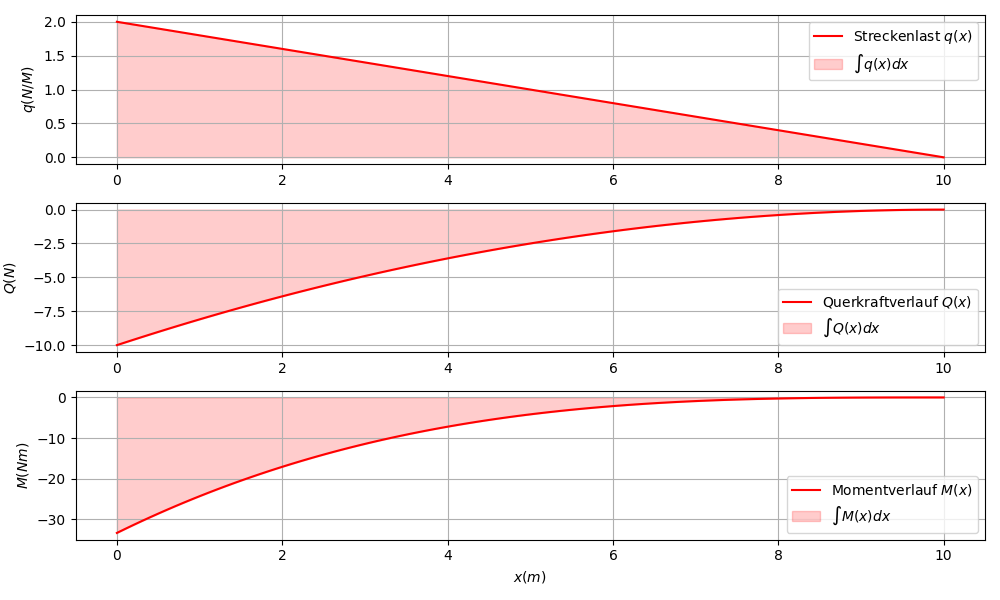
\includegraphics[width=\textwidth]{images/internal_forces_plot.png}
    \caption{Graphen für $q(x)$ in $\frac{N}{m}$, $Q(x)$ in $N$ und $M(x)$ in $Nm$ für $q_0=2, l=10$}
    \label{fig:InternalForcesPlot}
\end{figure}

\subsection{Fazit}
Die dargestellten Graphen (\ref{fig:InternalForcesPlot}) zeigen den Verlauf der Streckenlast $q(x)$, der Querkraft $Q(x)$ und des Moments $M(x)$ entlang eines Trägers mit einer Länge von $l = 10$ Metern und einer linear verteilten Streckenlast von $q_0 = 2$ Newton pro Meter. 

Die Analyse des Verhaltens eines Trägers unter linear abnehmender Streckenlast ist ein klassisches Problem in der Bauingenieurwissenschaft und bietet wertvolle Einblicke in die Tragwerksdynamik. Man erkennt, dass die Streckenlast $q(x)$, die linear von $q_0$ auf null am Ende des Trägers abfällt, zu einer Querkraft $Q(x)$ führt, die eine quadratische Abhängigkeit zeigt, und zu einem Biegemoment $M(x)$ , das kubisch mit $x$ ansteigt.

Die Ergebnisse zeigen, wie die Kräfte entlang des Trägers verlaufen. Die Querkraft beginnt bei $x=0$ mit dem Maximum und fällt zum Ende hin ab, was darauf hindeutet, dass der Träger an seinem fest geschweißten Ende die größte Belastung erfährt. Das Moment hat einen kubischen Verlauf, der vom maximalen Moment gegen null läuft, was die zunehmende Biegung des Trägers unter der Last verdeutlicht.

Die numerische Integration, also durch die Newton-Cotes-Formeln, hlft diese Verläufe anzunähern und per Code zu analysieren, wenn Zurückgreifen auf analoge Methoden nicht praktikabel ist. Dies ist besonders nützlich in komplizierten realen Anwendungsfällen, wo Lastverteilungen variieren oder nicht standardmäßige Geometrien eine Rolle spielen.
	
	%\chapter{Simpson-Formel, Varianten sowie Unterschiede und wo welche Simpson Formel sinnvoll ist}

\section{Varianten}

Bei der Simpson Regel gibt es vier verschiedene Varianten, welche nochmal in zwei Kategorien aufgeilt werden können. Man kann es in die \(\frac{1}{3}\)-Formel und die \(\frac{3}{8}\)-Formel unterteilen. Diese kann man dann wiederrum in die Einfache Simpson-\(\frac{1}{3}\)-Formel und die Zusammengesetzte Simpson-\(\frac{1}{3}\)-Formel, sowie die Einfache-\(\frac{3}{8}\)-Formel und die Zusammengesetzte Simpson-\(\frac{3}{8}\)-Formel unterteilen \textsc{\cite[S. 342]{SimpsonVarianten}}  \textsc{\cite[S. 327]{BasicNumMath}}.


\section{Unterschiede}\label{Unterschiede}

Bei den Unterschieden kann man ebenfalls wieder in die zwei Kategorien \(\frac{1}{3}\)-Formel und \(\frac{3}{8}\)-Formel unterteilen. Die Einfache Simpson-\(\frac{1}{3}\)-Formel kann man für ein einzelnes Intervall benutzen, welches in zwei gleich große Teile geteilt wurde. Die Zusammengesetzte Simpson-\(\frac{1}{3}\)-Formel kann man dahingegen für ein Intervall nutzen, welches in mehrere gleich große Teile geteilt wurde, wobei die Anzahl durch zwei teilbar sein muss. Bei den \(\frac{3}{8}\)-Formeln ist das so ähnlich, bis auf enen kleinen Unterschied. Die Einfache-\(\frac{3}{8}\)-Formel nutzt man für ein einzelnes Intervall, welches in drei gleich große Teile geteilt wurde und die Zusammengesetzte Simpson-\(\frac{3}{8}\)-Formel nutzt man für ein Intervall, das in mehrere gleich große Teile geteilt wurde, allerdings muss die Anzahl der Teile hierbei durch drei teilbar sein \textsc{\cite[S. 310]{NumMathe}} \textsc{\cite[S. 180]{NumMethodsScienceEng}}.


\section{Unter welchen Bedingungen bzw. Anforderungen ist welche Simpson Formel sinnvoll}

Im allgemeinen dienen die Simpson-Formeln dazu, eine höhere Genauigkeit zu erreichen als beispielsweise mit der Rechtecks- oder Trapezberechnung. \textsc{\cite[S. 310]{NumMathe}} Sofern die Abstände der Punkte gleichmäßig sind, kann man Formeln, wie die Simpson-Formeln, höherer Ordnung anwenden. Sowohl die \(\frac{1}{3}\)-Formel und die \(\frac{3}{8}\)-Formel haben die gleiche Genauigkeit. Man kann die Simpson-Formeln allerdings nicht nutzen, wenn die Punkte nicht gleichmäßig vertielt sind \textsc{\cite[S. 186]{NumMethodsScienceEng}}. Wie bei den Unterschieden \ref{Unterschiede} erwähnt, kann man die \(\frac{1}{3}\)-Formel dafür benutzen, um eine Fläche in einem Intervall zu berechnen, welche aus einer geraden Anzahl von Teilintervallen besteht. Hierbei muss man allerdings darauf achten, dass die Einfache Simpson-\(\frac{1}{3}\)-Formel nur zwei Teilintervalle haben darf, dafür aber die Zusammengesetzte Simpson-\(\frac{1}{3}\)-Formel aus mehreren Teilintervallen bestehen darf, diese Anzahl aber durch zwei teilbar sein muss. Bei der \(\frac{3}{8}\)-Formel ist das ähnlich, aber mit drei. Die Einfache Simpson-\(\frac{3}{8}\)-Formel muss aus drei Teilintervallen bestehen und die Zusammengesetzte Simpson-\(\frac{3}{8}\)-Formel muss aus einer Anzahl an Teilintervallen bestehen, welche durch drei Teilbar ist \textsc{\cite[S. 180]{NumMethodsScienceEng}} \textsc{\cite[S. 186]{NumMethodsScienceEng}}. 








 %Ist in Chapter Newton_Cotes_Formel
	
	%\include{}

    %\include{}

    %\include{}

    %\include{}
	
%%%%%%%%%%%%%%%%%%%%%%%%%%%%%%%%%%%%%%%%%%%%%%%%%%%%%%%%%%%%%%%%%%%%%%%%%%%%%%%%%%%%%%%%%%%%%%%%%%

    %%%%%%%%%%%%%%%%%%%
	%Abschluss
	%%%%%%%%%%%%%%%%%%%
    \section*{Abschluss}

Diese Hausarbeit gewährt eine breit gefächerte Untersuchung der praktischen, sowie theoretischen Aspekte der Integral- und Differentialrechnung, vor allem im Kontext von Computational Engineering. Durch eine detailierte Beschreibung und Analyse der FDM und der NCF wird ein tiefes Verständnis für die numerischen Verfahren zur Lösung von Differential- und Integralrechnungen vermittelt. Des Weiteren zeieigt die Implementierung dieser Methoden in Python, die praktische Anwendbarkeit und Flexibilität von modernen numerischen Techniken. Schlussendlich lässt sich somit festhalten, dass die in dieser Arbeit behandelten Methoden, sowie Ansätze unverzichtbare Werkzeuge für Wissenschaftler und Ingenieuere darstellen, um komplizierte Probleme in der realen Welt zu analysieren und zu lösen.
 
	%%%%%%%%%%%%%%%%%%%
	%Abbildungs- und Tabellenverzeichnis
	%%%%%%%%%%%%%%%%%%%
	\listoffigures % Abbildungsverzeichnis (captions in den Figuren werden als Referenz genommen)
	%\listoftables % Verzeichnis der Tabellen (captions in den Tabellen werden als Referenz genommen)
	
	%%%%%%%%%%%%%%%%%%%
	%Literaturverzeichnis an dieser Stelle
	%%%%%%%%%%%%%%%%%%%
	\printbibliography % Erstellt die Bibliography

\end{document}